\subsection{Définition}
Le terme « transcription musicale automatique » a été utilisé pour la première fois par les chercheurs en audio James A. Moorer, Martin Piszczalski et Bernard Galler en 1977. Grâce à leurs connaissances en ingénierie audio numérique, ces chercheurs pensaient qu'un ordinateur pouvait être programmé pour analyser un enregistrement numérique de musique de manière à détecter les hauteurs des lignes mélodiques et des motifs d'accords, ainsi que les accents rythmiques des instruments à percussion.\\La tâche de transcription automatique de la musique comprend deux activités distinctes : l'analyse d'un morceau de musique et l'impression d'une partition à partir de cette analyse.\\
\textit{Source : \url{https://en.wikipedia.org/wiki/Transcription_(music)}}
\subsection{Architecture générale}
La figure suivante, qui est une proposition de Benetos et Al. \cite{article1}, représente l'architecture générale d'un système de transcription musicale.\\\\
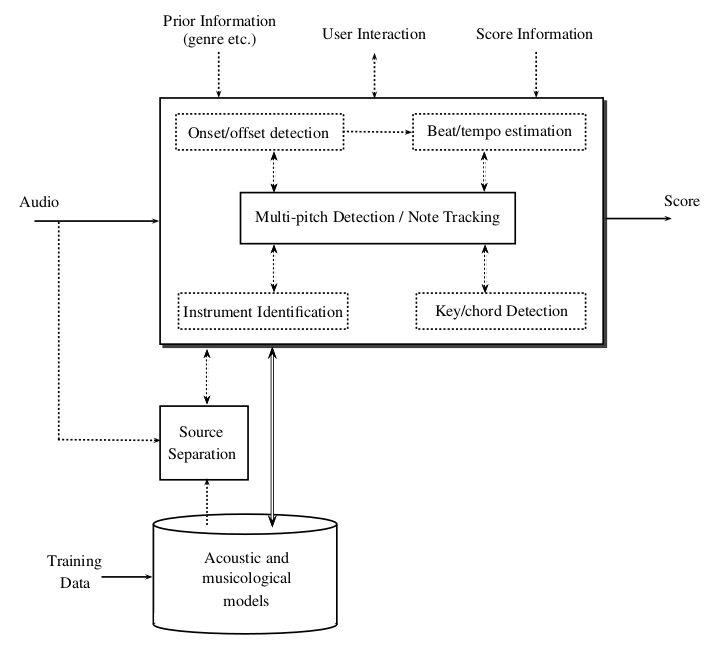
\includegraphics[height=60mm, width=60mm]{z_images/1_automatic_transcription/0_general_process.png}\\\\
\textit{Les sous-systèmes et algorithmes optionnels sont présentés à l'aide de lignes pointillées. Les doubles flèches mettent en évidence les connexions entre les systèmes qui incluent la fusion d'informations et une communication plus interactive entre les systèmes.}\\\\
Au cœur du système se trouvent les algorithmes de détection des multi-pitchs et de suivi des notes. Quatre sous-tâches de transcription liées à la détection des hauteurs multiples et au suivi des notes apparaissent comme des algorithmes facultatifs du système (cases en pointillé) qui peuvent être intégrés dans un système de transcription. Il s'agit de l'identification de l'instrument, de l'estimation de la tonalité et de l'accord, de la détection de l'apparition et du décalage, et de l'estimation du tempo et du rythme. La séparation des sources, un problème indépendant mais lié, pourrait être traitée par un système séparé qui pourrait informer et interagir avec le système de transcription en général, et plus spécifiquement avec le sous-système d'identification des instruments.
En option, des informations peuvent également être fournies de manière externe au système de transcription. Elles peuvent être données sous forme d'informations préalables (c'est-à-dire le genre, l'instrumentation, etc.), via l'interaction de l'utilisateur ou en fournissant des informations à partir d'une partition préexistante partiellement correcte ou incomplète. Enfin, les données de formation peuvent être utilisées pour apprendre des modèles acoustiques et musicologiques qui, par la suite, informent le système de transcription et interagissent avec lui. avec le système de transcription.
%\subsection{Exemple pour deux instruments}
%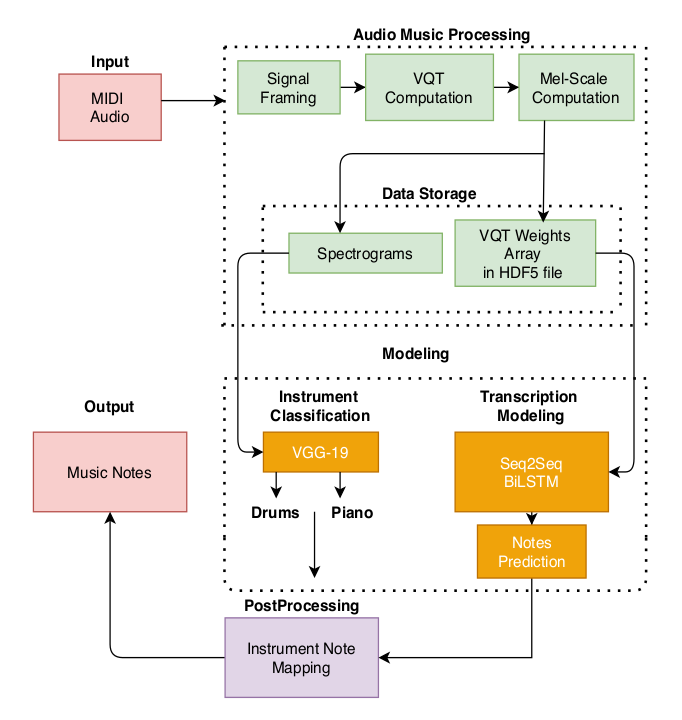
\includegraphics[height=60mm, width=60mm]{z_images/1_automatic_transcription/1_general_2instrus.png}\\
%\cite{article2}
%\subsection{Qparse}
%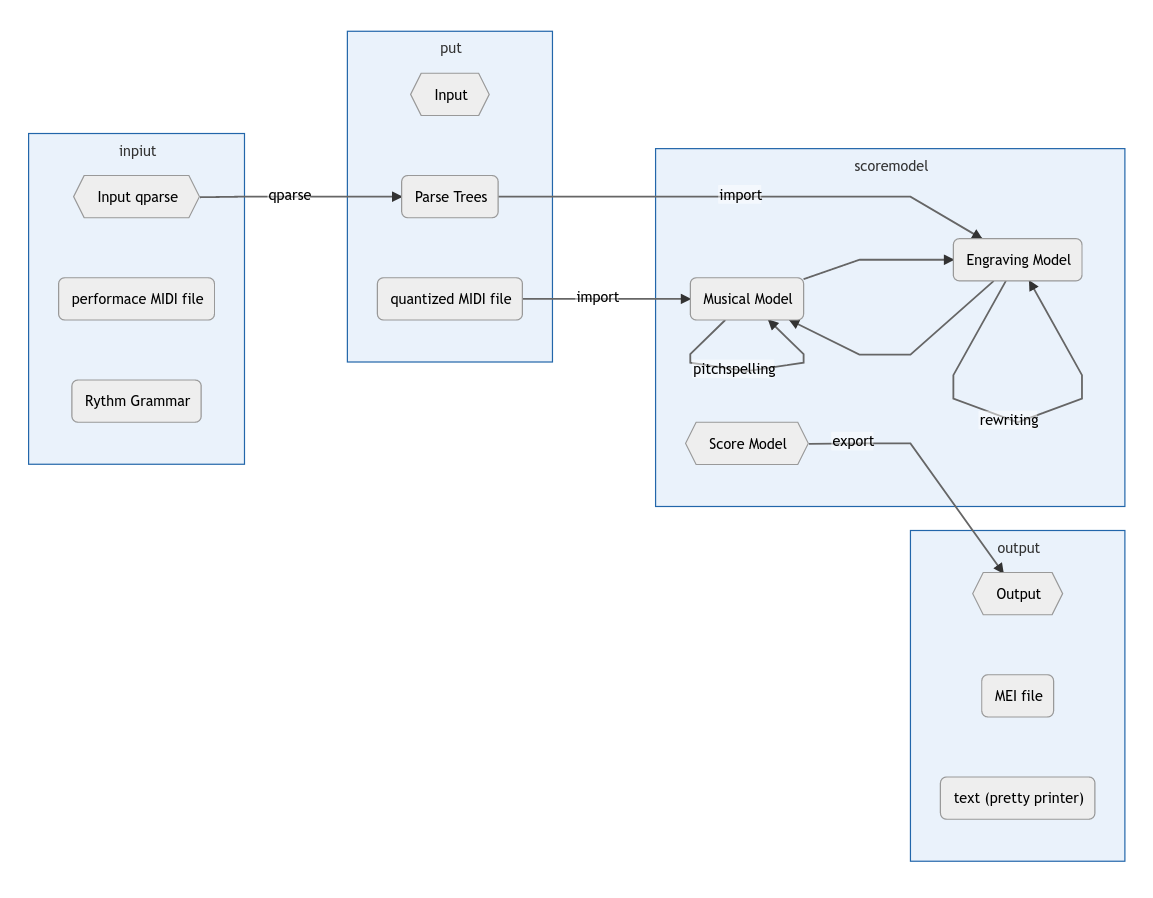
\includegraphics[height=60mm, width=60mm]{z_images/1_automatic_transcription/2_general_qparse.png}
